%As mentioned in section \ref{sec:bg}, the built-in deadlock detector (if not disabled \cite{go-netDeadlock}) only detects global deadlocks where the main goroutine is blocked and ignores other goroutines' states. For instance, more than 70\% of blocking bugs (partial deadlocks and leaks) in GoKer \cite{yuan-gobench-cgo21} are not detectable by the built-in deadlock detector.
%
As we have shown in our previous work \cite{parlot,difftrace}, dynamic tracing is an effective way in debugging large-scale applications.
%
We found that Go execution tracer \cite{go-cmd-trace} gives detailed information about the \textit{performance} behavior during execution.
%
Its tracing capability is compiled into all programs always through the runtime and is enabled on demand -- when tracing is disabled, it has minimal runtime overhead \cite{go-exec-tracer-doc}.
%
An execution model from the interactions of processors, OS threads, goroutines, the scheduler, and the garbage collection mechanism is constructible from the trace to identify poor parallelization and resource contention.
%
By enriching the tracer package with concurrency events, we place the missing pieces for human debuggers and analysis tools to automatically obtain comprehensive models from the dynamic concurrency behavior of programs with minimal overhead.
%
In the remainder of this section, we briefly describe the enhancement that we made to the tracer package to automatically obtain Execution Concurrency Trace (ECT) from program execution reflecting accurate behavior of Go concurrency primitives in section \ref{sec:ect} (overhead and scalability report is available in \cite{ect-arxiv}).
%
Then in section \ref{sec:dld}, we explain how we exploit ECT contents for post-mortem debugging of the program.
%
Sections \ref{sec:dl_instrument} and \ref{sec:dl_evaluation} provide more details on implementation and evaluation of deadlock detection using program ECT.

\begin{table}[]
    \centering
        \begin{tabular}{|l|l|}
        \hline
        \rowcolor[HTML]{C0C0C0}
        \multicolumn{1}{|c|}{\cellcolor[HTML]{C0C0C0}\textbf{Category}} & \multicolumn{1}{c|}{\cellcolor[HTML]{C0C0C0}\textbf{Description}} \\ \hline
        Process & Indication of process/thread start and stop \\ \hline
        GC/Mem & Garbage collection and memory operation events\\ \hline
        Goroutine & Goroutines events: create, block, start, stop, end, etc. \\ \hline
        Syscall & Interactions with system calls \\ \hline
        Users & User annotated regions and tasks (for bounded tracing) \\ \hline
        Misc & System related events like futile wakeup or timers \\ \hline
        \end{tabular}

    \caption{Event categories by the Go execution tracer}
    \label{tab:events}
\end{table}




\subsection{Execution Concurrency Tracing (ECT)}
\label{sec:ect}
%\stcmtside{why we need to mutate ET to ECT}
According to \cite{tu-concurrentBugs-asplos19,yuan-gobench-cgo21}, the primary cause of most real-world bugs is the misuse of concurrency features like channels, mutexes, and waitGroups (table \ref{tab:comparison}).
%
However, the standard tracer package does not capture concurrency primitive usage events as it aims more on performance bugs.
%
Although the event vocabulary is rich enough to model comprehensive goroutine latency and blocking behavior accurately, the tracer package cannot answer questions such as do the synchronization constructs work as expected? In the leaky interleaving of listing \ref{listing:moby28462.minipage}, which goroutine is holding the lock that \texttt{Monitor} tends to acquire? What are the resources that contribute to this circular wait? In the successful interleaving of listing \ref{listing:moby28462.minipage}, is there any \textit{potential flaw} that did not manifest?

%
%\stcmtside{why we think dynamic tracing is effective}
As we mentioned earlier, dynamic tracing provides a practical and uniform way to answer the above debugging questions and track multiple program facets during execution.
%
In the context of Go, we implemented a framework that automatically captures dynamic concurrency behavior exploiting an enhancement to the tracer package.
%
We chose the tracer package to enhance because it 1) is already compiled into the runtime, 2) adds minimal overhead, and 3) only lacks some pieces allowing the construction of an accurate concurrency model.
%

When enabled, the execution tracer package from the standard Go captures and compresses an \textit{execution concurrency trace} (ECT).
%
Upon program termination, the ECT is flushed to an IO buffer.
%
The decompressed ECT is a totally ordered \textit{sequence} of events in which the order is approximated through a central clock with nanosecond precision.
%
ECT also contains the call-stack for each event enabling a direct mapping of events to source-line numbers.
%
The alphabet of ECT is total of 63 events -- 49 from original tracer package \cite{goParserSource}, categorized and summarized in table \ref{tab:events} and 14 additional events that we added to capture concurrency usage events:
%
\begin{itemize}
    \item \textbf{Channel:} For each channel operation (make, send, receive, close), ECT includes an event with a unique id assigned to each channel.
    \item \textbf{(RW)Mutex, WaitGroup \& Conditional Variables:} Similar to channels, we assign a unique id to each concurrency object and emit an event for each of their operations (lock, unlock, rlock, runlock, add, wait, signal, broadcast).
    \item \textbf{Select \& Schedule:} The scheduler and the \textit{select} structure introduce non-determinism to the execution. We keep track of the decisions made by the scheduler and select statements to obtain an accurate decision path during execution.
\end{itemize}

%\stcmtside{how ECT captures concurrency blocking behavior}
Blocking concurrency operations such as channels \textit{sends}/\textit{recvs}, mutex \textit{locks}, waitGroup/conditional variable \textit{wait} and \textit{select} (when none of the cases are available) prevents the executor goroutine from making progress.
%
For each blocking operation, ECT captures a pair of pre-operation and post-operation events to distinguish between the \textit{request for action} and \textit{completion of action}.
%
ECT enables concurrency state modeling at any given step of execution through a replay of the sequence of events.
%

\subsection{Deadlock Detection}
\label{sec:dld}
We take advantage of the rich collection of information about the dynamic behavior of within ECT to automatically identify whether one or more goroutines have been leaked after program termination.
%
Upon program termination, we construct a goroutine tree (figure \ref{fig:gtree}) of application goroutines by replaying through the execution ECT.
%
In the goroutine tree, parents are the goroutines that children are created from within them. Each node of the tree contains information about the goroutine creation site, the resources that it holds at each execution point and the final executed event right before program termination.
%
In the lifetime of a program, the runtime system creates new goroutines or pick from the pool of dead goroutines to perform various tasks such as bootstrapping the program, garbage marking and sweeping, and tracing.
%
\goat also adds extra goroutine to \textit{watch} the main goroutine in case of blockage of the main goroutine.
%
These extra goroutines are captured in the tracing but we are not interested in studying them as our main focus is the main application (or test) and all application-level goroutines.
%
By checking the stack of creation location, \goat prune the goroutine and only keep the \textit{application-level} goroutines.
%
We say a goroutine is an application-level goroutine if it is the main goroutine (that executes the main function) or it has all of the following conditions:
1) its ancestor is the main goroutine,
2) it is not a Go runtime system goroutine, and
3) it is not a tracer goroutine.
Such distinguishment between goroutines is essential to define the boundaries of the application and the underlying system.

\begin{figure}[]
\centering
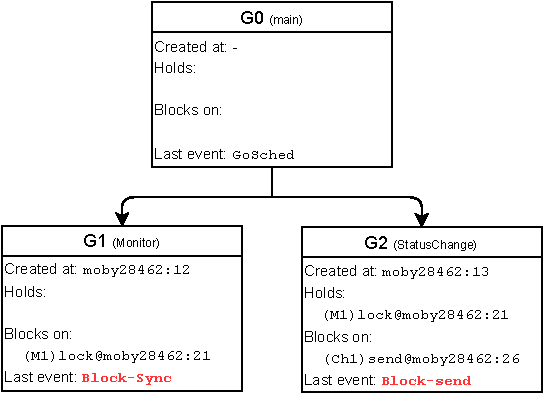
\includegraphics[width=0.75\linewidth]{figs/gtree.pdf}
%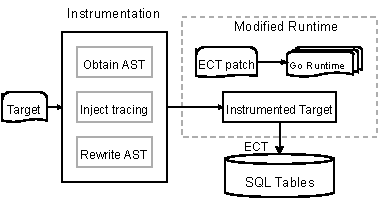
\includegraphics[]{figs/overview.png}
%\includegraphics[]{figs/overv}
\caption{Goroutine tree of the leaky interleaving in listing \ref{listing:moby28462}}
\label{fig:gtree}
\end{figure}

%
In addition to the parent/children relation of goroutines, nodes of the goroutine tree contains information about the goroutine creation site, the resources that it holds at each execution point and the final executed event right before program termination.
%
When tracing is enabled, every application goroutine invokes the tracer to capture $GoEnd$ before finishing its execution and exit (\ie change status from \textit{grunnable} to \textit{gdead}\cite{goexit-line-of-code}).
%
Before the main function returns, it calls the scheduler (through \texttt{runtime.Gosched()} invocation which captures $GoSched$ event) to hand over the control to the root goroutine to finish up program execution.
%
Since we instrument the application to call \texttt{runtime.traceStop} to stop tracing when main returns, $GoSched$ would be the last event captured for the main goroutine if it returns succesfully.
%

We call an execution \textbf{successful}, if below conditions hold
\begin{enumerate}
  \item (1) all goroutines spawned in the main goroutine has $GoEnd$ as their final event
  \item (2) the final event of the main goroutine is $GoSched$ with \texttt{runtime.traceStop} on top of its stack.
\end{enumerate}
If either of above conditions does not satisfy after program execution, a \textbf{deadlock} happens because it shows that there are one or more goroutine that did not reach its final state. \goat executes procedure \ref{proc:deadlockCheck} which is a BFS traversal on the goroutine tree to check if the program suffers from deadlocks.

\begin{small}
\begin{algorithm}[]
 \DontPrintSemicolon
 \SetKwFunction{KwDeadlockCheck}{DeadlockCheck}
% \SetKwInOut{Input}{Input} \SetKwInOut{Output}{Output}\SetKwInOut{Local}{Local}
  %\SetKw{KwEach}{each}
 %\Input{Stack of elements $S$, $S[1]$ is top}
 %\Output{$NLR(T)$}
 \KwDeadlockCheck{$G$}:{\\
 \Indp
    \If{$cur$.lastEvent$ \neq$ \texttt{GoSched}}{
      return \textbf{Global Deadlock}\;
    }
    $toVisit$ = $[G.children]$\;
    \For{ $|toVisit| \neq 0$}{
         $cur$ = $toVisit$[0]\;
         \If{$cur$.lastEvent $\neq$ \texttt{GoEnd}}{
            return \textbf{Partial Deadlock (leak)}\;
          }
         \For {$n$ in $cur.Children$}{
            append $n$ to $toVisit$\;
          }
          $toVisit = toVisit[1:]$\;
      }
      return \textbf{Pass}\;
  }
 \caption{\texttt{DeadlockCheck} procedure with root node of goroutine tree (main goroutine) as input}
 \label{proc:deadlockCheck}
\end{algorithm}
\end{small}



\begin{table*}[]
\caption{Output of each debugging tool after experimenting on bug for GoKer \cite{yuan-gobench-cgo21} blocking bugs. For each tool, here is how to interprete its output: Detected bug (minimum \# of executions required) -- \textbf{X (1000)} means that the tool is not able to detect any bug after 1000 executions. \textbf{PDL}: Partial Deadlock, \textbf{GDL}: Global Deadlock, \textbf{PDL-k}: Partial Deadlock with \textit{k} number of goroutines leaked. \textbf{DL}: A warning for potential deadlock is issued. \textbf{TO/GDL}: The global deadlock is detected because none of goroutines made any progress after 20 seconds, \textbf{CRASH}: The execution paniced because of a flaw in the execution (e.g., send on closed channels panic), \textbf{HANG}: The tool halt for more than 10 minutes.}
\centering
\scalebox{0.75}{
    % Please add the following required packages to your document preamble:
% \usepackage{multirow}
% \usepackage[table,xcdraw]{xcolor}
% If you use beamer only pass "xcolor=table" option, i.e. \documentclass[xcolor=table]{beamer}
\begin{tabular}{|c|c|c|ccc|ccccc|}
\hline
\multicolumn{3}{|c|}{Bug Description} & \multicolumn{8}{c|}{Debugging Tools} \\ \hline
 &  &  & \multicolumn{1}{c|}{} & \multicolumn{1}{c|}{} &  & \multicolumn{5}{c|}{GOAT} \\ \cline{7-11}
\multirow{-2}{*}{Cause} & \multirow{-2}{*}{SubCause} & \multirow{-2}{*}{Bug ID} & \multicolumn{1}{c|}{\multirow{-2}{*}{BUILTINDL}} & \multicolumn{1}{c|}{\multirow{-2}{*}{GOLEAK}} & \multirow{-2}{*}{LOCKDL} & \multicolumn{1}{c|}{D0} & \multicolumn{1}{c|}{D1} & \multicolumn{1}{c|}{D2} & \multicolumn{1}{c|}{D3} & D4 \\ \hline
 &  & cockroach\_2448 & X (1000) & X (1000) & X (1000) & CRASH (1) & CRASH (1) & CRASH (1) & CRASH (1) & CRASH (1) \\ \cline{3-3}
 &  & cockroach\_24808 & GDL (1) & GDL (1) & TO/GDL (1) & TO/GDL (1) & TO/GDL (1) & TO/GDL (1) & TO/GDL (1) & TO/GDL (1) \\ \cline{3-3}
 &  & cockroach\_25456 & GDL (1) & GDL(1) & TO/GDL (1) & TO/GDL (1) & TO/GDL (1) & TO/GDL (1) & TO/GDL (1) & TO/GDL (1) \\ \cline{3-3}
 &  & cockroach\_35073 & GDL (1) & GDL (1) & TO/GDL (1) & TO/GDL (1) & TO/GDL (1) & TO/GDL (1) & TO/GDL (1) & TO/GDL (1) \\ \cline{3-3}
 &  & cockroach\_35931 & GDL (1) & GDL (1) & TO/GDL (1) & TO/GDL (1) & TO/GDL (1) & TO/GDL (1) & TO/GDL (1) & TO/GDL (1) \\ \cline{3-3}
 &  & etcd\_6857 & X (1000) & PDL (325) & X (1000) & \cellcolor[HTML]{EFEFEF}PDL-1 (1) & \cellcolor[HTML]{EFEFEF}PDL-1 (1) & \cellcolor[HTML]{EFEFEF}PDL-1 (11) & \cellcolor[HTML]{EFEFEF}PDL-1 (3) & \cellcolor[HTML]{EFEFEF}PDL-1 (3) \\ \cline{3-3}
 &  & grpc\_1275 & X (1000) & PDL (1) & X (1000) & PDL-1 (1) & PDL-1 (1) & PDL-1 (1) & PDL-1 (1) & PDL-1 (1) \\ \cline{3-3}
 &  & grpc\_1424 & X (1000) & PDL (1) & X (1000) & PDL-1 (1) & PDL-1 (1) & PDL-1 (1) & PDL-1 (1) & PDL-1 (1) \\ \cline{3-3}
 &  & grpc\_660 & X (1000) & PDL (1) & X (1000) & PDL-1 (1) & PDL-1 (1) & PDL-1 (1) & PDL-1 (1) & PDL-1 (1) \\ \cline{3-3}
 &  & istio\_17860 & X (1000) & PDL (1) & X (1000) & PDL-1 (2) & PDL-1 (1) & PDL-1 (1) & PDL-1 (1) & PDL-1 (1) \\ \cline{3-3}
 &  & kubernetes\_38669 & X (1000) & PDL (1) & X (1000) & PDL-1 (1) & PDL-1 (1) & PDL-1 (1) & PDL-1 (1) & PDL-1 (1) \\ \cline{3-3}
 &  & kubernetes\_5316 & X (1000) & PDL (1) & X (1000) & PDL-1 (1) & PDL-2 (1) & PDL-1 (1) & PDL-2 (1) & PDL-2 (1) \\ \cline{3-3}
 &  & kubernetes\_70277 & GDL (1) & GDL (1) & TO/GDL (1) & TO/GDL (1) & TO/GDL (1) & TO/GDL (1) & TO/GDL (1) & TO/GDL (1) \\ \cline{3-3}
 &  & moby\_21233 & X (1000) & PDL (1) & X (1000) & PDL-2 (1) & PDL-2 (1) & PDL-2 (1) & PDL-2 (1) & PDL-2 (1) \\ \cline{3-3}
 &  & moby\_33293 & X (1000) & PDL (1) & X (1000) & PDL-1 (1) & PDL-1 (3) & PDL-1 (1) & PDL-1 (1) & PDL-1 (1) \\ \cline{3-3}
 &  & moby\_4395 & X (1000) & PDL (1) & X (1000) & PDL-1 (1) & PDL-1 (1) & PDL-1 (1) & PDL-1 (1) & PDL-1 (1) \\ \cline{3-3}
 & \multirow{-17}{*}{Channel} & syncthing\_5795 & GDL (1) & GDL (1) & TO/GDL (1) & TO/GDL (1) & TO/GDL (1) & TO/GDL (1) & TO/GDL (1) & TO/GDL (1) \\ \cline{2-11}
 &  & kubernetes\_11298 & X (1000) & X (1000) & TO/GDL (179) & X (1000) & TO/GDL (352) & TO/GDL (158) & TO/GDL (179) & TO/GDL (179) \\ \cline{3-3}
 & \multirow{-2}{*}{\begin{tabular}[c]{@{}c@{}}Channel   \&\\      Conditional Variable\end{tabular}} & moby\_27782 & X (1000) & PDL (741) & X (1000) & X (1000) & \cellcolor[HTML]{EFEFEF}PDL-2 (1) & \cellcolor[HTML]{EFEFEF}PDL-2 (1) & \cellcolor[HTML]{EFEFEF}PDL-2 (4) & \cellcolor[HTML]{EFEFEF}PDL-2 (4) \\ \cline{2-11}
 &  & cockroach\_10790 & X (1000) & PDL (3) & X (1000) & PDL-2 (1) & PDL-2 (1) & PDL-2 (1) & PDL-2 (1) & PDL-2 (1) \\ \cline{3-3}
 &  & cockroach\_13197 & X (1000) & PDL (1) & X (1000) & PDL-1 (1) & PDL-1 (1) & PDL-1 (1) & PDL-1 (1) & PDL-1 (1) \\ \cline{3-3}
 &  & cockroach\_13755 & X (1000) & PDL (1) & X (1000) & PDL-1 (1) & PDL-1 (1) & PDL-1 (1) & PDL-1 (1) & PDL-1 (1) \\ \cline{3-3}
 &  & cockroach\_18101 & X (1000) & PDL (1) & X (1000) & PDL-1 (1) & PDL-1 (1) & PDL-1 (1) & PDL-1 (1) & PDL-1 (1) \\ \cline{3-3}
 &  & grpc\_862 & X (1000) & PDL (1) & X (1000) & PDL-1 (1) & PDL-1 (1) & PDL-1 (1) & PDL-1 (1) & PDL-1 (1) \\ \cline{3-3}
 &  & istio\_18454 & X (1000) & PDL (13) & X (1000) & PDL-2 (5) & PDL-1 (14) & PDL-1 (4) & PDL-1 (6) & PDL-1 (6) \\ \cline{3-3}
 &  & kubernetes\_25331 & X (1000) & PDL (1) & X (1000) & PDL-1 (1) & PDL-1 (1) & PDL-1 (1) & PDL-1 (1) & PDL-1 (1) \\ \cline{3-3}
 & \multirow{-8}{*}{\begin{tabular}[c]{@{}c@{}}Channel \& \\      Context\end{tabular}} & moby\_33781 & X (1000) & PDL (1) & X (1000) & PDL-1 (221) & PDL-1 (10) & PDL-1 (8) & PDL-1 (10) & PDL-1 (10) \\ \cline{2-11}
 &  & moby\_29733 & GDL (1) & GDL (1) & TO/GDL (1) & TO/GDL (1) & TO/GDL (1) & TO/GDL (1) & TO/GDL (1) & TO/GDL (1) \\ \cline{3-3}
\multirow{-29}{*}{\begin{tabular}[c]{@{}c@{}}Communication\\       Deadlock\end{tabular}} & \multirow{-2}{*}{Condition Variable} & moby\_30408 & GDL (1) & GDL (1) & TO/GDL (1) & TO/GDL (1) & TO/GDL (1) & TO/GDL (1) & TO/GDL (1) & TO/GDL (1) \\ \hline
 &  & etcd\_6873 & X (1000) & PDL (371) & X (1000) & PDL-2 (1) & PDL-2 (2) & PDL-2 (7) & PDL-2 (6) & PDL-2 (6) \\ \cline{3-3}
 &  & etcd\_7443 & X (1000) & X (1000) & X (1000) & X (1000) & \cellcolor[HTML]{EFEFEF}PDL-1 (9) & \cellcolor[HTML]{EFEFEF}PDL-1 (15) & \cellcolor[HTML]{EFEFEF}PDL-1 (14) & \cellcolor[HTML]{EFEFEF}PDL-1 (14) \\ \cline{3-3}
 &  & etcd\_7492 & HANG (1) & HANG (1) & TO/GDL (4) & TO/GDL (1) & TO/GDL (1) & TO/GDL (1) & TO/GDL (1) & TO/GDL (1) \\ \cline{3-3}
 &  & etcd\_7902 & X (1000) & PDL (1) & X (1000) & PDL-4 (1) & PDL-4 (1) & PDL-4 (1) & PDL-4 (1) & PDL-4 (1) \\ \cline{3-3}
 &  & grpc\_1353 & X (1000) & PDL (1) & X (1000) & CRASH (1) & CRASH (1) & PDL-3 (1) & PDL-3 (1) & PDL-3 (1) \\ \cline{3-3}
 &  & grpc\_1460 & X (1000) & PDL (1) & X (1000) & PDL-2 (135) & PDL-2 (1) & PDL-2 (2) & PDL-2 (1) & PDL-2 (1) \\ \cline{3-3}
 &  & istio\_16224 & GDL (1) & GDL (1) & TO/GDL (1) & TO/GDL (1) & TO/GDL (1) & TO/GDL (1) & TO/GDL (1) & TO/GDL (1) \\ \cline{3-3}
 &  & kubernetes\_10182 & X (1000) & PDL (44) & X (1000) & \cellcolor[HTML]{EFEFEF}PDL-2 (1) & \cellcolor[HTML]{EFEFEF}PDL-2 (1) & \cellcolor[HTML]{EFEFEF}PDL-2 (1) & \cellcolor[HTML]{EFEFEF}PDL-2 (1) & \cellcolor[HTML]{EFEFEF}PDL-2 (1) \\ \cline{3-3}
 &  & kubernetes\_1321 & X (1000) & PDL (307) & X (1000) & X (1000) & \cellcolor[HTML]{EFEFEF}PDL-1 (1) & \cellcolor[HTML]{EFEFEF}PDL-1 (1) & \cellcolor[HTML]{EFEFEF}PDL-1 (1) & \cellcolor[HTML]{EFEFEF}PDL-1 (1) \\ \cline{3-3}
 &  & kubernetes\_26980 & GDL (375) & GDL (131) & X (1000) & TO/GDL (191) & TO/GDL (1) & TO/GDL (1) & TO/GDL (1) & TO/GDL (1) \\ \cline{3-3}
 &  & kubernetes\_6632 & X (1000) & X (1000) & X (1000) & \cellcolor[HTML]{EFEFEF}PDL-2 (1) & \cellcolor[HTML]{EFEFEF}PDL-2 (1) & \cellcolor[HTML]{EFEFEF}PDL-2 (2) & \cellcolor[HTML]{EFEFEF}PDL-2 (1) & \cellcolor[HTML]{EFEFEF}PDL-2 (1) \\ \cline{3-3}
 &  & moby\_28462 & X (1000) & PDL (5) & X (1000) & PDL-2 (39) & PDL-2 (1) & PDL-2 (1) & PDL-2 (1) & PDL-2 (1) \\ \cline{3-3}
 & \multirow{-13}{*}{Channel \& Lock} & serving\_2137 & X (1000) & X (1000) & X (1000) & X (1000) & X (1000) & TO/GDL (88) & X (1000) & X (1000) \\ \cline{2-11}
 &  & cockroach\_1055 & GDL (1) & GDL (1) & TO/GDL (1) & TO/GDL (1) & TO/GDL (1) & TO/GDL (1) & TO/GDL (1) & TO/GDL (1) \\ \cline{3-3}
 & \multirow{-2}{*}{\begin{tabular}[c]{@{}c@{}}Channel   \& \\      WaitGroup\end{tabular}} & cockroach\_1462 & X (1000) & X (1000) & TO/GDL (1) & X (1000) & TO/GDL (1) & TO/GDL (1) & TO/GDL (1) & TO/GDL (1) \\ \cline{2-11}
\multirow{-16}{*}{\begin{tabular}[c]{@{}c@{}}Mixed \\      Deadlock\end{tabular}} & Misuse WaitGroup & moby\_25384 & X (1000) & PDL (1) & X (1000) & PDL-1 (1) & PDL-1 (1) & PDL-1 (1) & PDL-1 (1) & PDL-1 (1) \\ \hline
 &  & cockroach\_584 & X (1000) & PDL (1) & X (1000) & PDL-1 (1) & PDL-1 (1) & PDL-1 (1) & PDL-1 (1) & PDL-1 (1) \\ \cline{3-3}
 &  & cockroach\_9935 & X (1000) & PDL (1) & DL (721) & PDL-1 (1) & PDL-1 (2) & PDL-1 (1) & PDL-1 (1) & PDL-1 (1) \\ \cline{3-3}
 &  & etcd\_10492 & GDL (1) & GDL (1) & DL (1) & TO/GDL (1) & TO/GDL (1) & TO/GDL (1) & TO/GDL (1) & TO/GDL (1) \\ \cline{3-3}
 &  & etcd\_5509 & X (1000) & GDL (766) & TO/GDL (426) & X (1000) & TO/GDL (1) & TO/GDL (1) & TO/GDL (1) & TO/GDL (1) \\ \cline{3-3}
 &  & etcd\_6708 & GDL (1) & GDL (1) & DL (1) & TO/GDL (1) & TO/GDL (1) & TO/GDL (1) & TO/GDL (1) & TO/GDL (1) \\ \cline{3-3}
 &  & grpc\_3017 & GDL (4) & GDL (4) & TO/GDL (3) & TO/GDL (1) & TO/GDL (1) & TO/GDL (1) & TO/GDL (1) & TO/GDL (1) \\ \cline{3-3}
 &  & grpc\_795 & GDL (1) & GDL (1) & DL (1) & TO/GDL (1) & TO/GDL (1) & TO/GDL (1) & TO/GDL (1) & TO/GDL (1) \\ \cline{3-3}
 &  & hugo\_5379 & GDL (1) & GDL (1) & TO/GDL (1) & TO/GDL (1) & TO/GDL (1) & TO/GDL (1) & TO/GDL (1) & TO/GDL (1) \\ \cline{3-3}
 &  & moby\_17176 & X (1000) & PDL (1) & X (1000) & PDL-1 (1) & PDL-1 (1) & PDL-1 (1) & PDL-1 (1) & PDL-1 (1) \\ \cline{3-3}
 &  & moby\_36114 & X (1000) & PDL (1) & X (1000) & PDL-1 (1) & PDL-1 (1) & PDL-1 (1) & PDL-1 (1) & PDL-1 (1) \\ \cline{3-3}
 &  & moby\_7559 & X (1000) & PDL (1) & X (1000) & PDL-1 (1) & PDL-1 (1) & PDL-1 (1) & PDL-1 (1) & PDL-1 (1) \\ \cline{3-3}
 & \multirow{-12}{*}{Double locking} & syncthing\_4829 & GDL (1) & GDL (1) & DL (1) & TO/GDL (1) & TO/GDL (1) & TO/GDL (1) & TO/GDL (1) & TO/GDL (1) \\ \cline{2-11}
 &  & cockroach\_16167 & X (1000) & X (1000) & DL (1) & X (1000) & TO/GDL (1) & TO/GDL (1) & TO/GDL (1) & TO/GDL (1) \\ \cline{3-3}
 &  & cockroach\_3710 & X (1000) & X (1000) & DL (123) & \cellcolor[HTML]{EFEFEF}PDL-2 (28) & \cellcolor[HTML]{EFEFEF}PDL-2 (1) & \cellcolor[HTML]{EFEFEF}PDL-2 (1) & \cellcolor[HTML]{EFEFEF}PDL-2 (1) & \cellcolor[HTML]{EFEFEF}PDL-2 (1) \\ \cline{3-3}
 &  & cockroach\_6181 & X (1000) & PDL (1) & X (1000) & PDL-4 (1) & PDL-4 (1) & PDL-3 (1) & PDL-1 (1) & PDL-1 (1) \\ \cline{3-3}
 &  & hugo\_3251 & GDL (1) & GDL (1) & DL (1) & TO/GDL (1) & TO/GDL (1) & TO/GDL (1) & TO/GDL (1) & TO/GDL (1) \\ \cline{3-3}
 &  & kubernetes\_58107 & X (1000) & X (1000) & X (1000) & \cellcolor[HTML]{EFEFEF}PDL-1 (1) & \cellcolor[HTML]{EFEFEF}PDL-1 (1) & \cellcolor[HTML]{EFEFEF}PDL-1 (1) & \cellcolor[HTML]{EFEFEF}PDL-1 (1) & \cellcolor[HTML]{EFEFEF}PDL-1 (1) \\ \cline{3-3}
 & \multirow{-6}{*}{RWR deadlock} & kubernetes\_62464 & X (1000) & X (1000) & DL (6) & PDL-2 (161) & PDL-2 (7) & PDL-2 (2) & PDL-2 (3) & PDL-2 (3) \\ \cline{2-11}
 &  & cockroach\_10214 & X (1000) & X (1000) & X (1000) & \cellcolor[HTML]{EFEFEF}PDL-2 (368) & \cellcolor[HTML]{EFEFEF}PDL-2 (1) & \cellcolor[HTML]{EFEFEF}PDL-2 (1) & \cellcolor[HTML]{EFEFEF}PDL-2 (1) & \cellcolor[HTML]{EFEFEF}PDL-2 (1) \\ \cline{3-3}
 &  & cockroach\_7504 & X (1000) & X (1000) & X (1000) & \cellcolor[HTML]{EFEFEF}PDL-2 (199) & \cellcolor[HTML]{EFEFEF}PDL-2 (1) & \cellcolor[HTML]{EFEFEF}PDL-2 (7) & \cellcolor[HTML]{EFEFEF}PDL-2 (1) & \cellcolor[HTML]{EFEFEF}PDL-2 (1) \\ \cline{3-3}
 &  & kubernetes\_13135 & X (1000) & PDL (1) & DL (4) & PDL-2 (1) & PDL-2 (5) & PDL-2 (1) & PDL-2 (22) & PDL-2 (22) \\ \cline{3-3}
 &  & kubernetes\_30872 & X (1000) & PDL (338) & X (1000) & \cellcolor[HTML]{EFEFEF}PDL-3 (50) & \cellcolor[HTML]{EFEFEF}PDL-3 (2) & \cellcolor[HTML]{EFEFEF}PDL-3 (1) & \cellcolor[HTML]{EFEFEF}PDL-3 (6) & \cellcolor[HTML]{EFEFEF}PDL-3 (6) \\ \cline{3-3}
\multirow{-23}{*}{\begin{tabular}[c]{@{}c@{}}Resource \\      Deadlock\end{tabular}} & \multirow{-5}{*}{AB-BA deadlock} & moby\_4951 & X (1000) & PDL (120) & X (1000) & \cellcolor[HTML]{EFEFEF}PDL-2 (15) & \cellcolor[HTML]{EFEFEF}PDL-2 (2) & \cellcolor[HTML]{EFEFEF}PDL-2 (2) & \cellcolor[HTML]{EFEFEF}PDL-2 (1) & \cellcolor[HTML]{EFEFEF}PDL-2 (1) \\ \hline
\multicolumn{1}{|l|}{Total Bugs:} & \multicolumn{1}{l|}{68} & \multicolumn{1}{l|}{Total Detected:} & 19 & 56 & 26 & 60 & 67 & 68 & 67 & 67 \\ \hline
\end{tabular}

  }
\label{tab:comparison}
\end{table*}



\subsection{Accelerating Bug Exposure}
\label{sec:critical}
As we have shown in figure \ref{fig:rare_bugs}, there are cases that the deadlock is hidden in the interleaving space.
%
It is proved that context-switches before synchronization/serialization operations in concurrent programs increases the probability of finding rare concurrent bugs \cite{burckhardt-depthBug-asplos10}.
%
For example, a rare context-switch right after the select statement in line \ref{bugListing:Monitor_select} causes the lock operation on mutex $m$ in line \ref{bugListing:Monitor_case_def_lock} of goroutine \texttt{Monitor} to \textit{block} goroutine \texttt{StatusChange} on locking $m$ in line \ref{bugListing:statChange_lock} and causing a deadlock.
%
Concurrency primitive usages are the \textit{critical points} in the program because their behavior directly impacts the blocking behavior of Go programs.
%
In \goat, we identify the usage of concurrency primitives as the critical points of the program before which a context-switch increases the probablity of manifesting a hidden bug that might not occur during conventional or stress testing.
%These critical points are interesting to study application correctness because 1)their behavior depends on the state of other goroutines at each execution step, 2) investigating their behavior and interaction with other goroutines is the key to debug the program behavior, 2) a contex-switch before their execution might change the operation behavior, and consequently the whole program behavior.
%
%
We define \textit{concurrency usage} (CU) as a triple of $<f,l,k>$ where $f$ is the file name, $l$ is the line number and $k$ is the kind of concurrency primitive used in the code location.
Kind $k\in$ \texttt{Channel} $\cup$ \texttt{Sync} $\cup$ \texttt{Go}:
\begin{itemize}
  \item \texttt{Channel} = \{\texttt{send}, \texttt{receive}, \texttt{close}\}
  \item \texttt{Sync} = \{\texttt{lock}, \texttt{unlock}, \texttt{wait}, \texttt{add}, \texttt{done}, \texttt{signal}, \texttt{broadcast}\}
  \item \texttt{Go} = \{\texttt{go}, \texttt{select}, \texttt{range}\}
\end{itemize}

The first column of table \ref{tab:moby_cov_table} shows the critical points extracted from program in listing \ref{listing:moby28462.minipage}.
%
We identify CU points by parsing the abstract syntax tree (AST) of the target source using Go AST package \cite{go-package-ast}.
%
CU points are passed to the instrumentation phase of \goat to inject scheduler perturbation handlers before these points.


\subsection{Instrumentation}
\label{sec:dl_instrument}

To equip the target application with concurrency tracing mechanism, we automatically inject three lines of code to the beginning of main or test function using AST package \cite{go-package-ast}:

\begin{itemize}
  \item \texttt{goat\_done := goat.Start()} initilizes \goat, enables tracing, and returns a channel as conduit between application space and \goat API.
  \item \texttt{go goat.Watch(goat\_done)} spawns a new goroutine as a watcher for liveness of the program (in case of global deadlocks or infinite loop). The watcher goroutine either receives from \texttt{goat\_done} and sends back an ack signal, or timeouts and stop tracing, and terminates.
  \item \texttt{defer goat.Stop(goat\_done)} sends a value to the watcher goroutine after main returns and signals that the program is finished. Then it waits to receive the signal from watcher, then stops tracing and terminates.
\end{itemize}

Additionally, to manipulate the native scheduler around CU points, we inject calls to \texttt{goat.handler()} before each statically discovered CU. \texttt{goat.handler()} randomly calls \texttt{runtime.GoSched()} to preempt the processing core from current goroutine and push the goroutine to the back of the global queue.



\begin{table}[]
\centering
\caption{Concurrency Usages and coverage requirements of program in listing\ref{listing:moby28462.minipage}}
\scalebox{0.9}{

\begin{tabular}{
>{\columncolor[HTML]{FFFFFF}}c
>{\columncolor[HTML]{FFFFFF}}l |
>{\columncolor[HTML]{FFFFFF}}l |
>{\columncolor[HTML]{FFFFFF}}c |
>{\columncolor[HTML]{FFFFFF}}c |
>{\columncolor[HTML]{FFFFFF}}c |}
\hline
\multicolumn{2}{|c|}{\cellcolor[HTML]{FFFFFF}CU of list. \ref{listing:moby28462.minipage}} & \multicolumn{1}{c|}{\cellcolor[HTML]{FFFFFF}} & \multicolumn{2}{c|}{\cellcolor[HTML]{FFFFFF}Covered by} & \cellcolor[HTML]{FFFFFF} \\ \cline{1-2} \cline{4-5}
\multicolumn{1}{|c|}{\cellcolor[HTML]{FFFFFF}Line} & \multicolumn{1}{c|}{\cellcolor[HTML]{FFFFFF}Kind} & \multicolumn{1}{c|}{\multirow{-2}{*}{\cellcolor[HTML]{FFFFFF}Coverage Requirements}} & run \#1 & run \#2 & \multirow{-2}{*}{\cellcolor[HTML]{FFFFFF}\begin{tabular}[c]{@{}c@{}}Overall\\      Covered\end{tabular}} \\ \hline
\multicolumn{1}{|c|}{\cellcolor[HTML]{FFFFFF}12} & go & covered & $\checkmark_{G0}$ & $\checkmark_{G0}$ & $\checkmark$ \\ \hline
\multicolumn{1}{|c|}{\cellcolor[HTML]{FFFFFF}13} & go & covered & $\checkmark_{G0}$ & $\checkmark_{G0}$ & $\checkmark$ \\ \hline
\multicolumn{1}{|c|}{\cellcolor[HTML]{FFFFFF}} & \cellcolor[HTML]{FFFFFF} & c-recv-blocked & $\checkmark_{G1}$ &  & $\checkmark$ \\ \cline{3-6}
\multicolumn{1}{|c|}{\multirow{-2}{*}{\cellcolor[HTML]{FFFFFF}17}} & \multirow{-2}{*}{\cellcolor[HTML]{FFFFFF}select} & c-recv-unblocking & $\checkmark_{G1}$ &  & $\checkmark$ \\ \hline
\multicolumn{1}{|c|}{\cellcolor[HTML]{FFFFFF}} & \cellcolor[HTML]{FFFFFF} & blocked &  & \cellcolor[HTML]{C0C0C0}$\checkmark_{G1}$ & $\checkmark$ \\ \cline{3-6}
\multicolumn{1}{|c|}{\multirow{-2}{*}{\cellcolor[HTML]{FFFFFF}21}} & \multirow{-2}{*}{\cellcolor[HTML]{FFFFFF}lock} & blocking & $\checkmark_{G1}$ &  & $\checkmark$ \\ \hline
\multicolumn{1}{|c|}{\cellcolor[HTML]{FFFFFF}} & \cellcolor[HTML]{FFFFFF} & unblocking & $\checkmark_{G1}$ &  & $\checkmark$ \\ \cline{3-6}
\multicolumn{1}{|c|}{\multirow{-2}{*}{\cellcolor[HTML]{FFFFFF}22}} & \multirow{-2}{*}{\cellcolor[HTML]{FFFFFF}unlock} & no\_op &  &  &  \\ \hline
\multicolumn{1}{|c|}{\cellcolor[HTML]{FFFFFF}} & \cellcolor[HTML]{FFFFFF} & blocked & $\checkmark_{G2}$ &  & $\checkmark$ \\ \cline{3-6}
\multicolumn{1}{|c|}{\multirow{-2}{*}{\cellcolor[HTML]{FFFFFF}25}} & \multirow{-2}{*}{\cellcolor[HTML]{FFFFFF}lock} & blocking &  & \cellcolor[HTML]{C0C0C0} \textbf{$\checkmark_{G2}$} & $\checkmark$ \\ \hline
\multicolumn{1}{|c|}{\cellcolor[HTML]{FFFFFF}} & \cellcolor[HTML]{FFFFFF} & blocked & $\checkmark_{G2}$ & $\checkmark_{G2}$ & $\checkmark$ \\ \cline{3-6}
\multicolumn{1}{|c|}{\cellcolor[HTML]{FFFFFF}} & \cellcolor[HTML]{FFFFFF} & unblocking &  &  &  \\ \cline{3-6}
\multicolumn{1}{|c|}{\multirow{-3}{*}{\cellcolor[HTML]{FFFFFF}26}} & \multirow{-3}{*}{\cellcolor[HTML]{FFFFFF}send} & no\_op &  &  &  \\ \hline
\multicolumn{1}{|c|}{\cellcolor[HTML]{FFFFFF}} & \cellcolor[HTML]{FFFFFF} & unblocking &  &  &  \\ \cline{3-6}
\multicolumn{1}{|c|}{\multirow{-2}{*}{\cellcolor[HTML]{FFFFFF}27}} & \multirow{-2}{*}{\cellcolor[HTML]{FFFFFF}unlock} & no\_op & $\checkmark_{G2}$ &  & $\checkmark$ \\ \hline
\multicolumn{1}{l}{\cellcolor[HTML]{FFFFFF}} &  & Coverage \% & 60\% & 33\% & 73\% \\ \cline{3-6}
\end{tabular}

}
\label{tab:moby_cov_table}
\end{table}


\subsection{Evaluation}
\label{sec:dl_evaluation}
In this section, we assess the ability of \goat and its variations in detecting bugs with minimum number of executions required to expose the bug.
%
We have compared \goat against three existing dynamic detectors:
\begin{itemize}
  \item \textit{Built-in} Deadlock Detector: It is an embeded mechanism in the standard Go runtime. The mechanism periodically makes sure that the queue of \textit{runnable} goroutines is never empty until the main goroutine terminates. If the queue is empty and main has not terminated yet (\ie main is blocked), it throws a runtime error.
  \item \textit{goleak} \cite{goleak}: This leak detector from Uber checks the program stack at the end of the main goroutine to find the application-level goroutines that remained in the stack (\ie leaked).
  \item \textit{LockDL} \cite{lockdl}: This tool intercept with all mutex locks and unlocks of the target application to maintain a ``lock-set'' data structure. \textit{LockDL} issues warning during runtime when it finds a circular wait in the lock-set or double-locking the same lock. It has a timeout mechanism for application that traps into global deadlocks (30 seconds by default).
\end{itemize}

All experiments are performed on a server with two AMD Ryzen 5 3600 6-Core Processor (12 total cores with 2 threads per core and 6 cores per socket), 64 GB of RAM with generic Ubuntu 4.15.0 and Go version 1.15.6.
%
Table \ref{tab:comparison} shows the details of results obtained from executing each tool per bug 1000 times.
%
We show that the tool is unable to detect the bug after 1000 executions with \textbf{X (1000)}.
%

%
Figure \ref{fig:detection} and table \ref{tab:comparison} show that variations of \goat outperforms other detector by discovering the bug in 100\% of the GoKer blocking benchmark.
%
Figure \ref{fig:runs} and highlighted cells of table \ref{tab:comparison} show that the idea of injecting random delays around concurrency usage points in the program drastically reduces the required number of testing iterations until the bug occur.
%
D0 means \goat did not delay the program at any point and D4 means that the target program has been delayed up to four times around its CU points.
%
Figures \ref{fig:detection} and \ref{fig:runs} also state that the increase in the delay bound of \goat does not necessarily increase the chance of exposing the bug.
%
For example, the row of bug \texttt{serving\_2137} in table \ref{tab:comparison} show that only \goat D2 were able to detect the bug.

\begin{figure}
\centering
  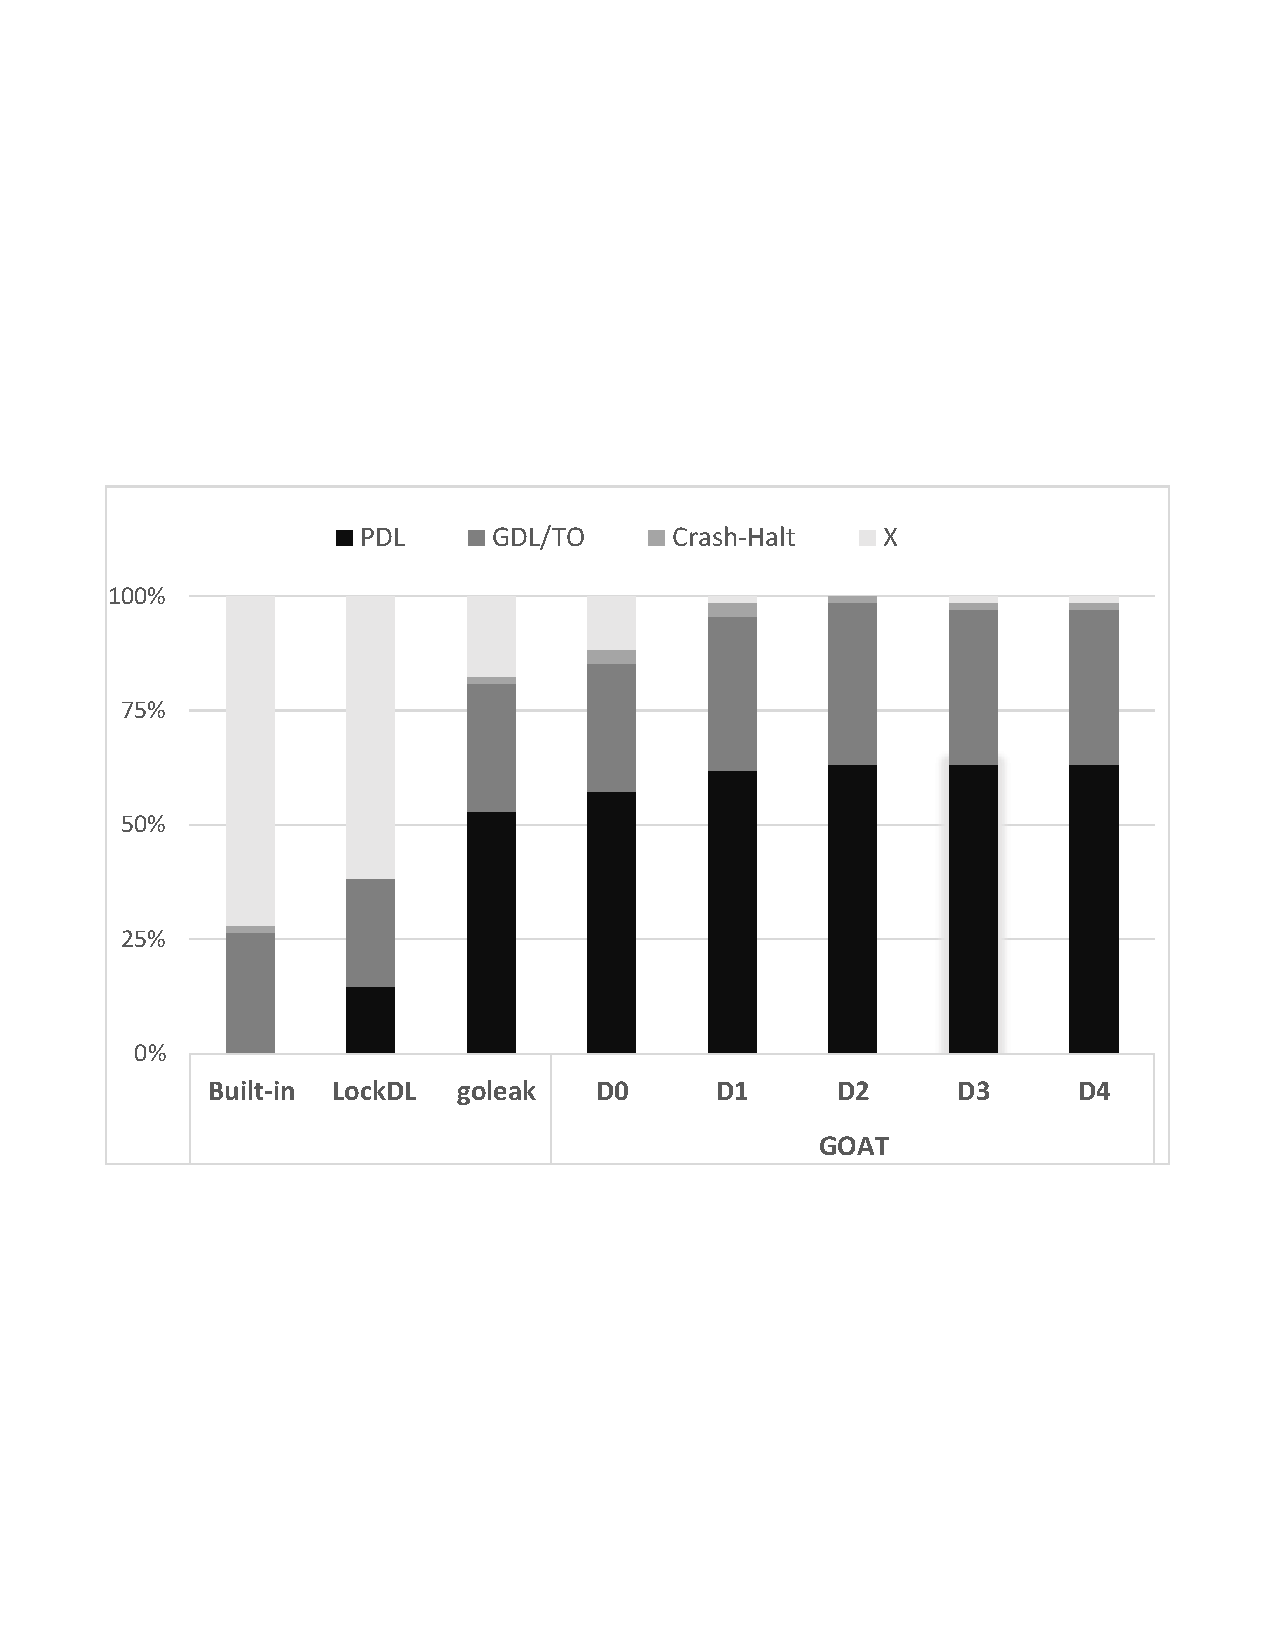
\includegraphics[width=.95\linewidth]{figs/P4_detections.pdf}
  \caption{Distribution of detected bugs by built-in deadlock detector (BUILTINDL), LockDL, GoLeak, and GOAT different D over 1000 runs. PDL: partial deadlock, GDL/TO: global deadlock, Crash/Halt: causes the program to crash or halt during detection, X: nothing is detected }
  \label{fig:detection}
\end{figure}


\begin{figure}
\centering
  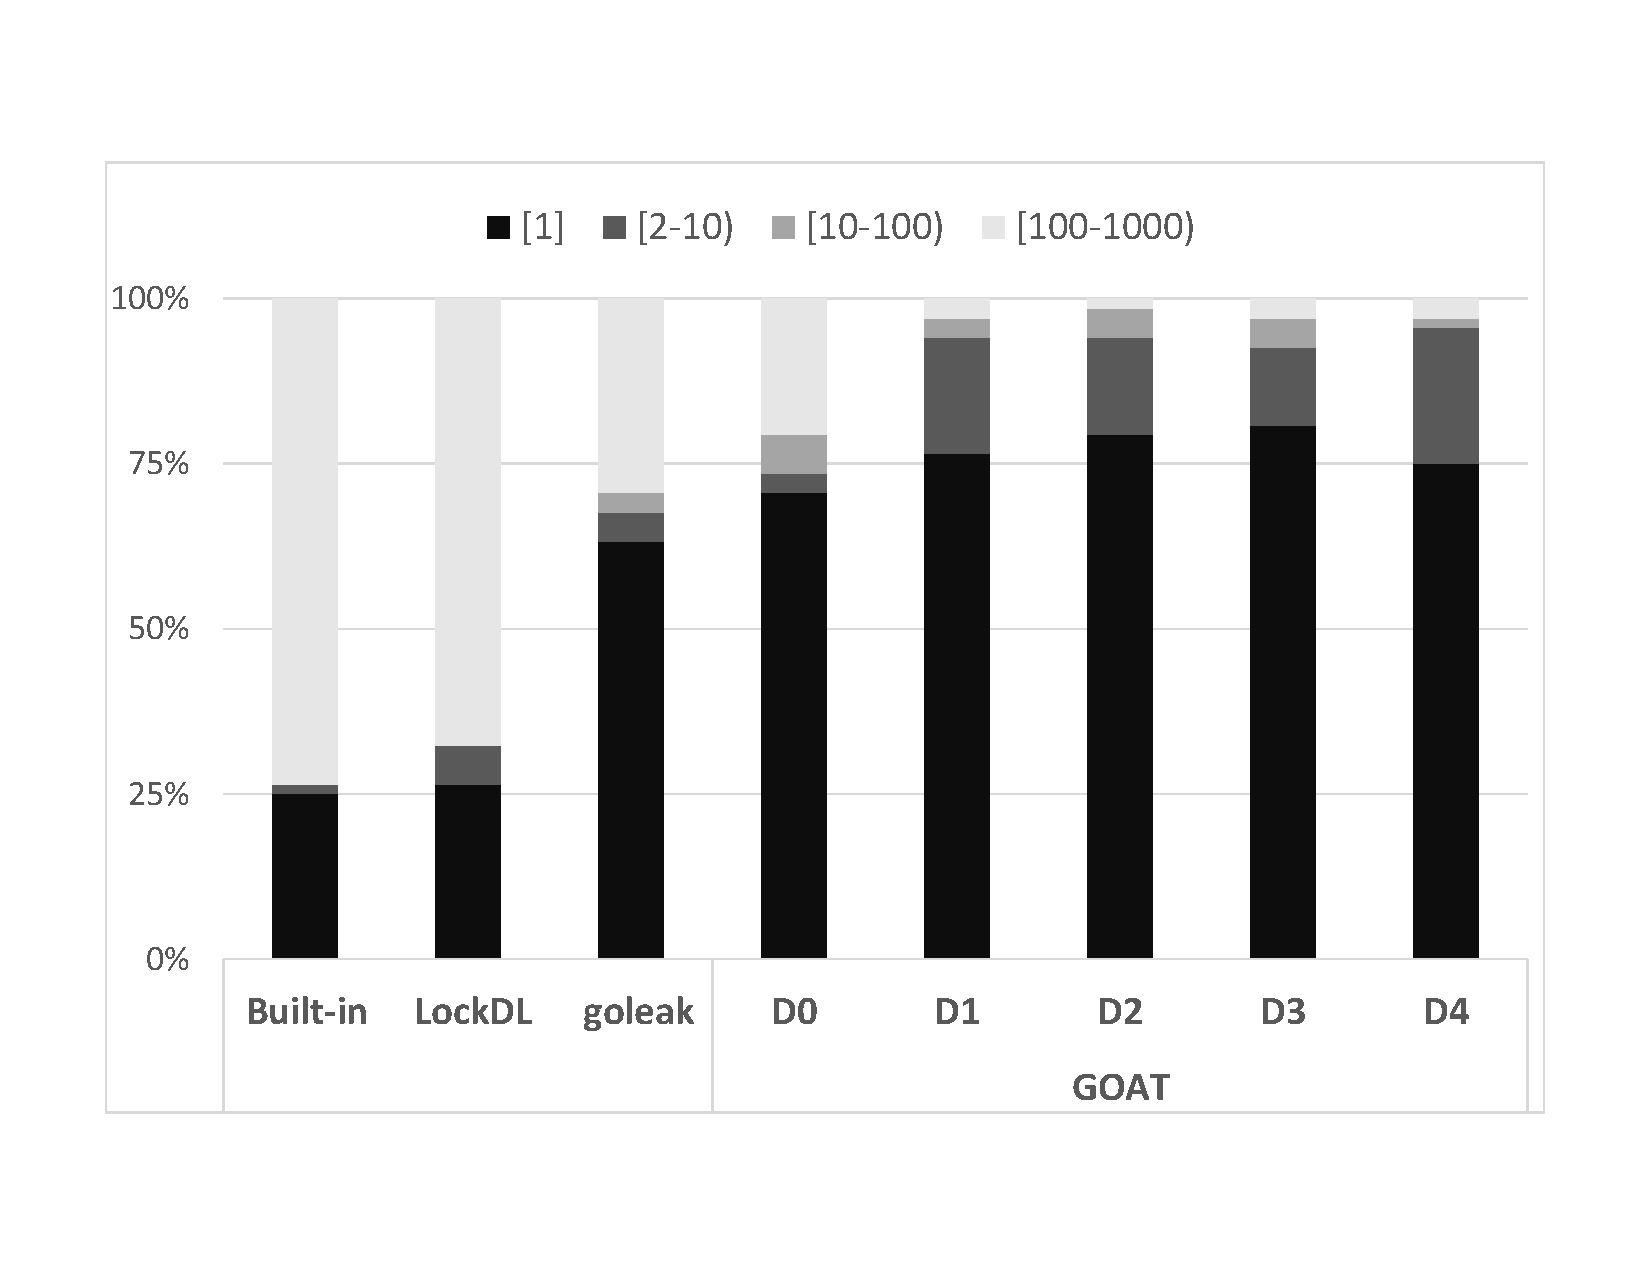
\includegraphics[width=.95\linewidth]{figs/P4_runs.pdf}
  \caption{Distribution of required number of iterations to detect the bug for each tool}
  \label{fig:runs}
\end{figure}
